% template for a task
% each task should be added to exactly one workpackage
% in the workpackage task list
\begin{task}[
  title=JupyterHub / BinderHub convergence,
  id=jh-bh-conv,
  lead=EP,
  PM=16, % EP: 12PM, WTT: 2PM, PSUD: 2PM
  wphases={0-36!.5},
  partners={WTT}]

  \textbf{Scenario}

  An institution -- typically a university, a national lab, a transnational
  research infrastructure such as the European XFEL, or transnational
  infrastructure provider like EGI, or even an NGO or SME -- wishes to provide its members and
  users with a Jupyter service.

  The service lets user spawn and access personal or collaborative virtual
  environments: namely a web interface to a light weight virtual machine,
  in which they can use Jupyter notebooks, run calculations, etc.

  \begin{figure}
    \begin{center}
      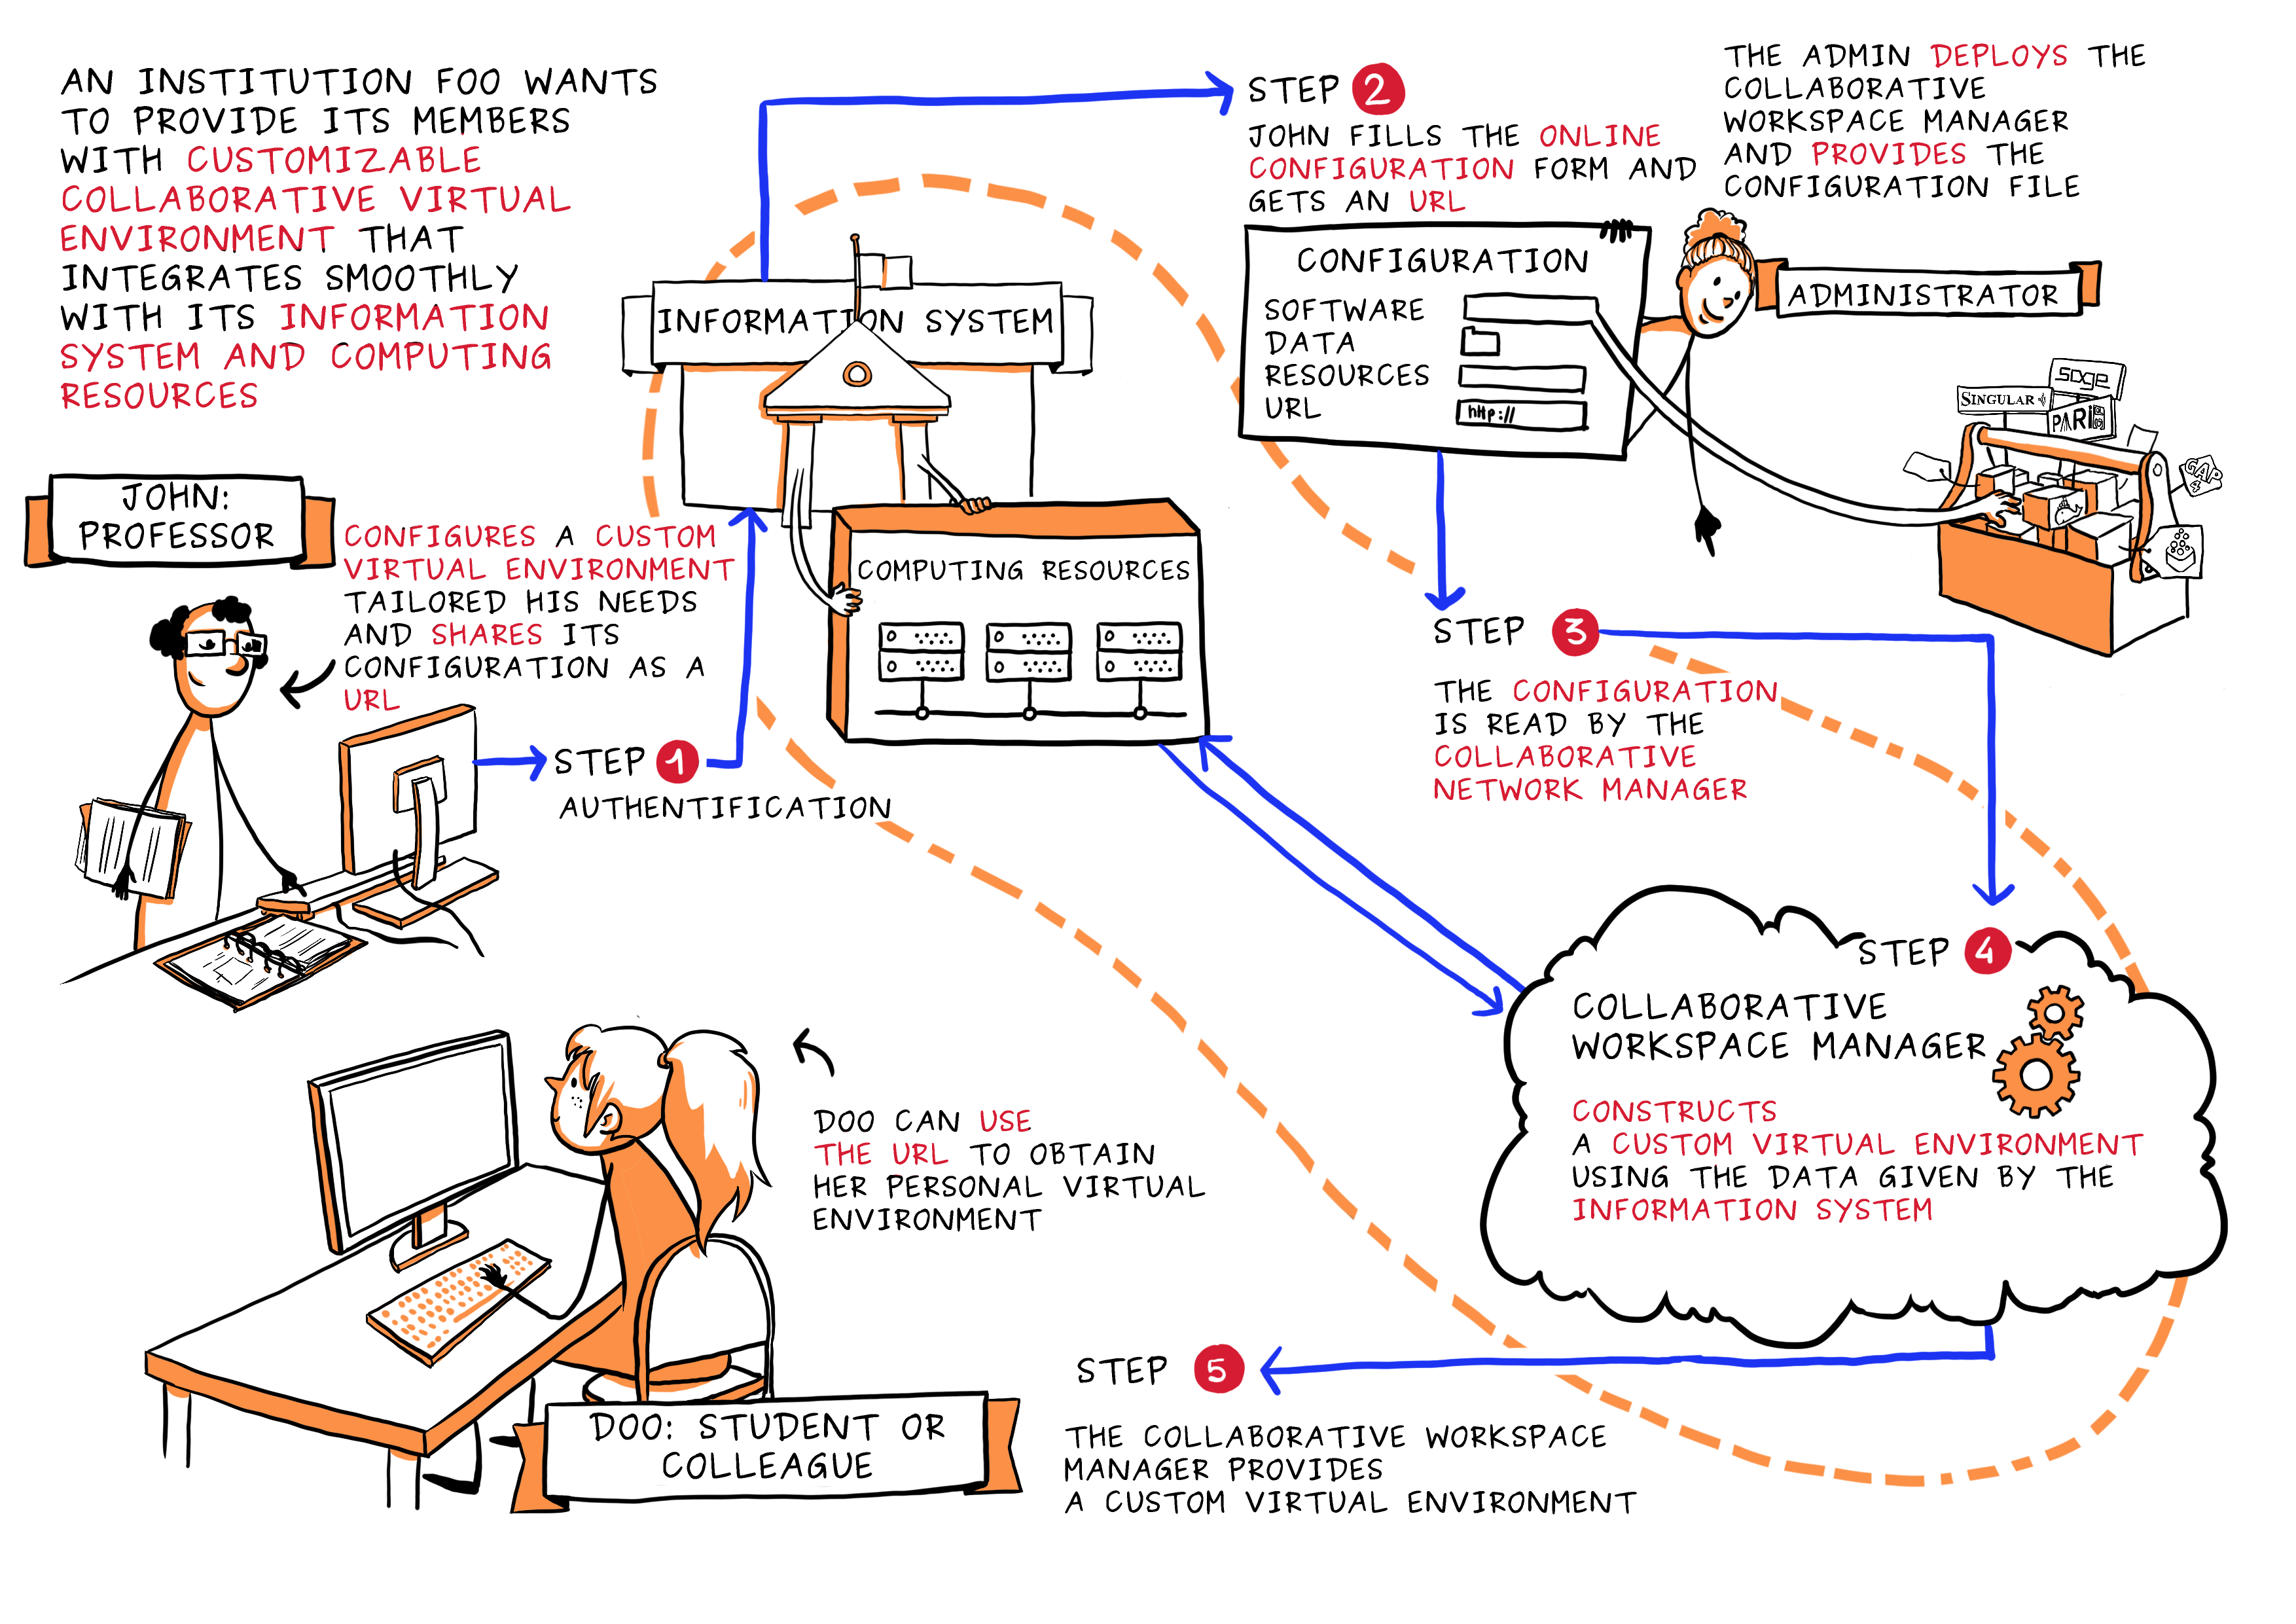
\includegraphics[width=.75\textwidth]{images/jupyterhub-binder-convergence.png}
    \end{center}
    \caption{Scenario for the JupyterHub - Binder convergence}
    \label{fig:jupyterhub-binder}
  \end{figure}

  To cater for a large variety of use cases in teaching and research,
  the main aim of the upcoming specifications is to make the service as
  versatile as possible. In particular, it should empower the users to 
  customize the service (available software stack, storage setup, ...),
  without a need for administrator intervention.

  \textbf{State of the art}
  JupyterHub already provides authentication, persistent storage and some
  default environments for its users. On the other hand, BinderHub offers
  the possibility to define more precisely the requirements for your teaching
  or research environment which makes it very flexible. However, BinderHub is still missing the  
  authentication and persistent storage capabilities provided by JupyterHub.

  \textbf{This task}
  The purpose of this task is to have the same services offered by JupyterHub
  (authentication, persistent storage, ...) with the flexibility of BinderHub
  (construction of your own environment for teaching or research).

  % Motivation: \TODO{reuse material from the blog post:
  % \url{https://opendreamkit.org/2018/03/15/jupyterhub-binder-convergence/}}
  % \TODO{reuse material from the hackmd notes with Tim:
  % \url{https://hackmd.io/0DLDCXcmRzC_dOwjEak3hg#}}
  The task includes the following activities:
  \begin{compactitem}
  \item Extend where needed JupyterHub's authentication features% (OIDC, ...)
  \item Credential management
  \item Customizable persistence at the admin, and user level
  \item Choice of container registry at the admin and user level % Could be moved to the repo2docker/binder task
  \item Runtime resource configuration % (disk, memory, cpus, time, ...)
  \end{compactitem}
  We will provide a report explaining how to make JupyterHub/Binder convergence a reality (\localdelivref{jh-bh-conv-report}).
\end{task}
